\section{Results}
\label{sec:results}

\subsection{Mechanistic Proof: Ratio Reward Advantage Variance (h-e1)}

\begin{table}[h]
\centering
\caption{Advantage comparison for illustrative GRPO group (8 completions, 5 test cases, group $[0,0,1,2,0,3,0,0]$).}
\label{tab:advantages}
\begin{tabular}{lccccc}
\toprule
\textbf{Completion} & \textbf{Test passes} & \textbf{Binary reward} & \textbf{Ratio reward} & \textbf{Binary adv.} & \textbf{Ratio adv.} \\
\midrule
c1 & 0/5 & 0.000 & 0.000 & 0.000 & $-$0.150 \\
c2 & 0/5 & 0.000 & 0.000 & 0.000 & $-$0.150 \\
c3 & 1/5 & 0.000 & 0.200 & 0.000 & $+$0.050 \\
c4 & 2/5 & 0.000 & 0.400 & 0.000 & $+$0.250 \\
c5 & 0/5 & 0.000 & 0.000 & 0.000 & $-$0.150 \\
c6 & 3/5 & 0.000 & 0.600 & 0.000 & $+$0.450 \\
c7 & 0/5 & 0.000 & 0.000 & 0.000 & $-$0.150 \\
c8 & 0/5 & 0.000 & 0.000 & 0.000 & $-$0.150 \\
\midrule
\textbf{Group mean} & --- & \textbf{0.000} & \textbf{0.150} & --- & --- \\
\textbf{Advantage variance} & --- & \textbf{0.0000} & \textbf{0.0475} & --- & --- \\
\bottomrule
\end{tabular}
\end{table}

This result is a mathematical guarantee. For this group --- in which 5 of 8 completions fail all tests, 2 achieve partial credit (1--2 passes), and 1 achieves 3 passes --- binary reward must produce zero gradient contribution. Ratio reward must produce non-zero gradient that pushes the model toward higher-$k$ completions. The advantage variance difference (0.0475 vs.\ 0.0000) is exact.

\subsection{Scale of the Dead Zone: 1,000-Group Simulation}

Figure~\ref{fig:histograms} shows the distribution of group-level advantage variance across 1,000 simulated early-training GRPO groups.

Under binary reward: 987/1,000 groups (98.7\%) have advantage variance = 0.0 --- all completions fail all tests. Only 13/1,000 groups (1.3\%) have non-zero binary reward variance (rare groups where at least one completion passes all 5 tests).

Under ratio reward: 987/1,000 groups (98.7\%) have advantage variance $> 0$ --- at least one completion achieves partial credit. Ratio reward provides learning signal in 98.7\% of early-training groups where binary reward provides none.

\begin{figure}[h]
\centering
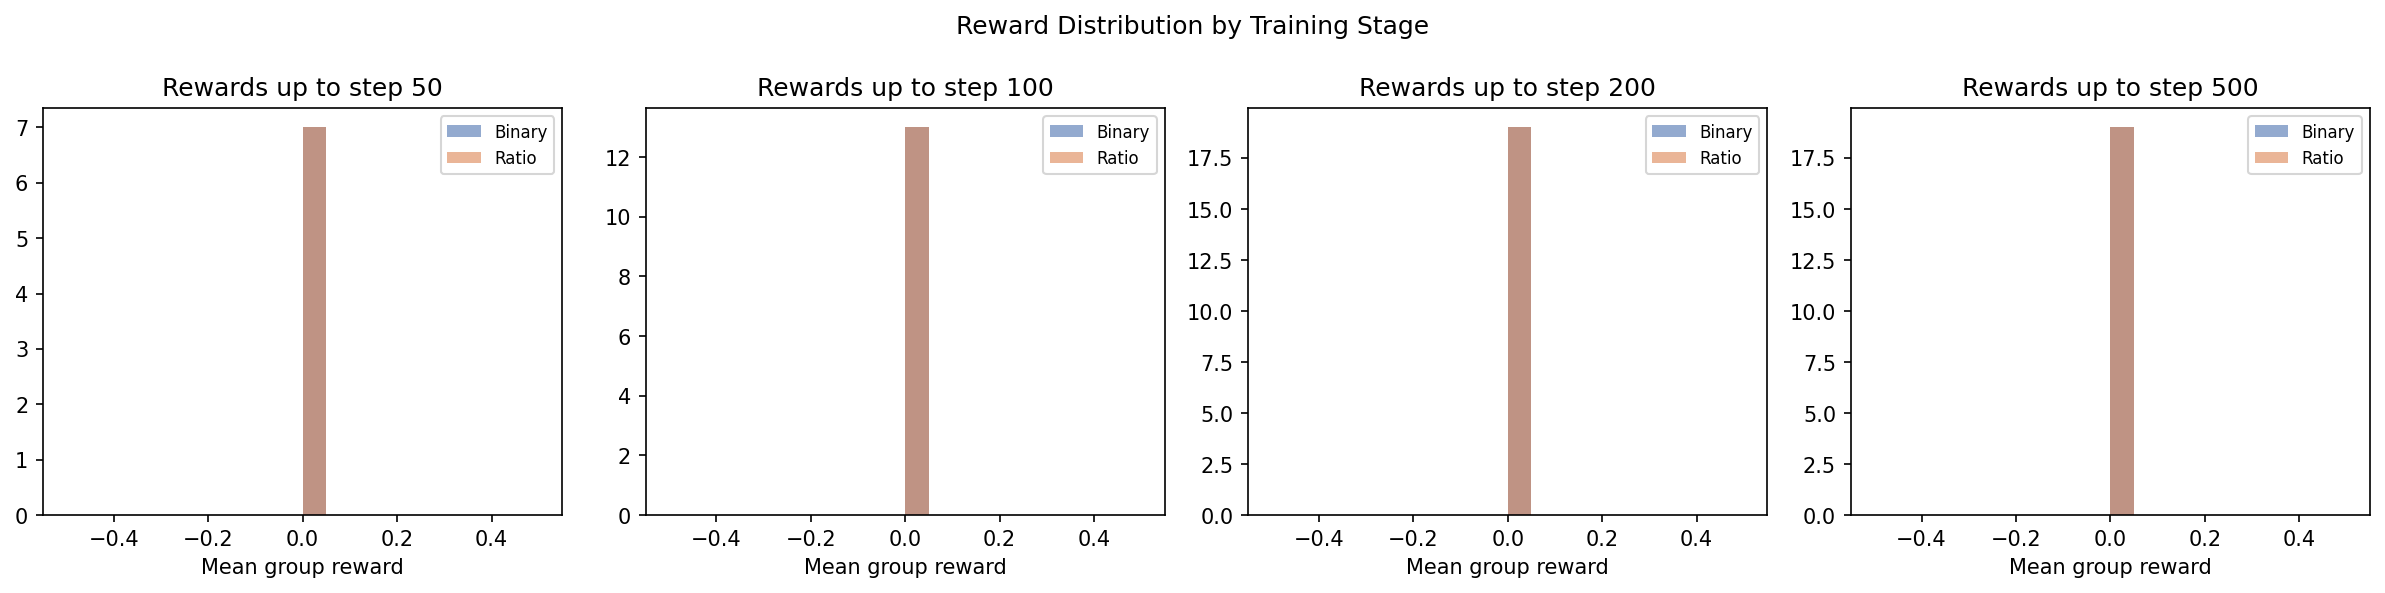
\includegraphics[width=0.85\columnwidth]{figures/reward_histograms.png}
\caption{Distribution of group-level advantage variance across 1,000 simulated early-training GRPO groups ($G=8$, $n=5$, $p_{\text{pass}}=0.1$). Binary reward (left): 98.7\% of groups have zero variance. Ratio reward (right): 98.7\% of groups have non-zero variance.}
\label{fig:histograms}
\end{figure}

\subsection{Infrastructure Validation}

Smoke test (3 GRPO steps, binary condition, GPU 0): exit code 0; gradient norms steps 1--3 in range $[3{\times}10^{-4}, 7{\times}10^{-4}]$; checkpoint saved. Duration: $\sim$54 sec/step on H100 NVL.\footnote{The h-e1 smoke test used \texttt{max\_new\_tokens=256} (fast validation configuration), while the h-m1 policy-level experiment used \texttt{max\_new\_tokens=512}. The gradient norms reported here reflect the 256-token smoke test.} Unit test results: 35/35 passing (h-e1: 17/17; h-m1: 18/18).

\subsection{h-m1 Training: Precision Null Result}

\begin{table}[h]
\centering
\caption{h-m1 training diagnostics (all 208 logged steps).}
\label{tab:hm1}
\begin{tabular}{lcc}
\toprule
\textbf{Metric} & \textbf{Binary} & \textbf{Ratio} \\
\midrule
reward\_mean & 0.0000 & 0.0000 \\
clipped\_ratio & 1.0000 & 1.0000 \\
fraction\_partial & NaN & NaN \\
mean\_terminated\_length & 0 & 0 \\
grad\_norm diff (ratio$-$binary, steps 1--136) & \multicolumn{2}{c}{mean: $+$0.000730; 95\% CI: [$-$0.000253, $+$0.002561]} \\
\bottomrule
\end{tabular}
\end{table}

Both conditions show \texttt{reward\_mean = 0.000} at all 208 logged training steps. \texttt{clipped\_ratio = 1.0} at all steps: every completion reaches the 512-token limit --- no completion generates a natural end-of-sequence token. \texttt{fraction\_partial = NaN}: no partial-pass completions were observed (the denominator is 0 throughout).

\textbf{Why both rewards are identical.} When no completion executes any test case (all completions are truncated non-programs), $r_{\text{binary}}(c) = 0$ and $r_{\text{ratio}}(c) = 0$ for all $c$. Both rewards are mathematically equivalent (both = 0 for all completions in all groups). GRPO produces zero gradient contribution from every group, for both conditions.

Figure~\ref{fig:gradnorm} shows per-step gradient norms for binary and ratio conditions. Both produce norms in $[0.5{\times}10^{-3}, 3{\times}10^{-3}]$, with no consistent directional difference. Gradient norm 95\% bootstrap CI on (ratio $-$ binary), steps 1--136: mean = $+$0.000730, CI = $[-$0.000253, $+$0.002561], includes zero --- consistent with both conditions receiving identical zero-reward gradients from the GRPO reward head.

\begin{figure}[h]
\centering
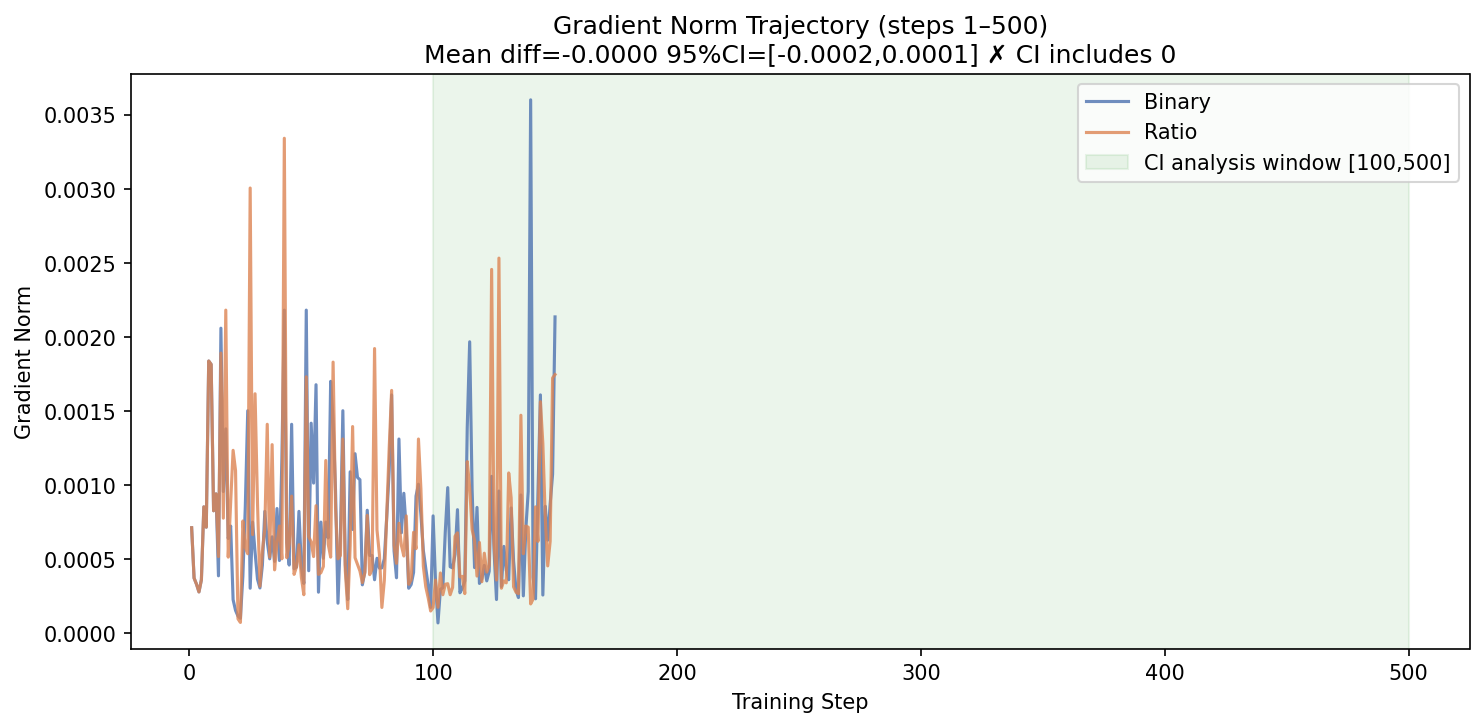
\includegraphics[width=0.85\columnwidth]{figures/grad_norm_trajectory.png}
\caption{Per-step gradient norms for binary and ratio conditions (h-m1, steps 1--136). Both conditions produce comparable norms with no consistent directional difference, consistent with identical zero-reward signals.}
\label{fig:gradnorm}
\end{figure}

\begin{figure}[h]
\centering
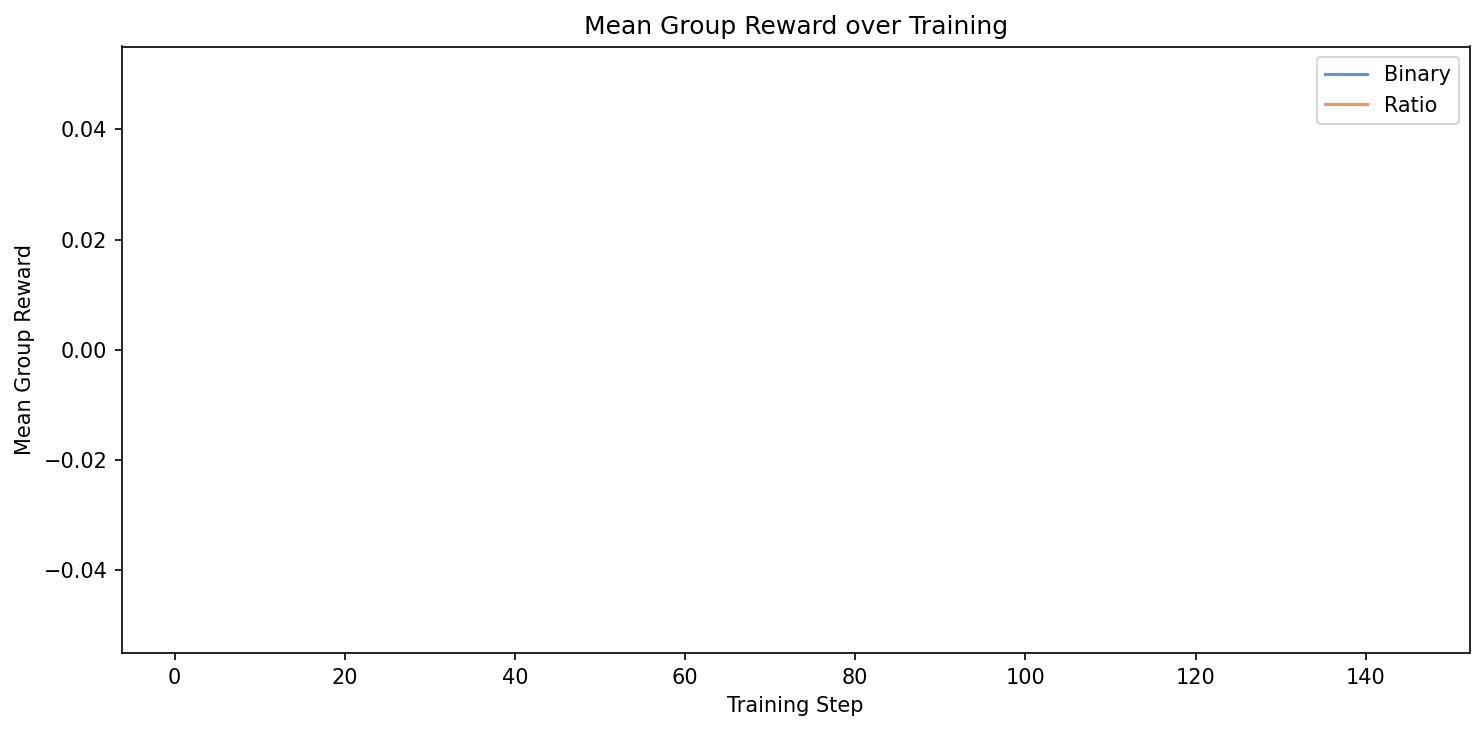
\includegraphics[width=0.85\columnwidth]{figures/mean_reward.png}
\caption{Reward mean trajectories for binary and ratio conditions across the h-m1 training run (208 logged steps). Both conditions remain at \texttt{reward\_mean = 0} throughout.}
\label{fig:meanreward}
\end{figure}

\textbf{Gate verdict: NOT SATISFIED.} Since both conditions are reward-equivalent (both = 0 throughout), no policy divergence can emerge. The experiment was terminated and routed to Phase 0 redesign.

\subsection{Summary}

\begin{table}[h]
\centering
\caption{Summary of experimental results.}
\label{tab:summary}
\begin{tabular}{lcc}
\toprule
\textbf{Result} & \textbf{Value} & \textbf{Status} \\
\midrule
Binary advantage variance (illustrative group) & 0.0000 & Mathematical guarantee \\
Ratio advantage variance (illustrative group) & 0.0475 & Mathematical guarantee \\
Groups receiving ratio$\neq$binary signal (simulation) & 987/1,000 (98.7\%) & Confirmed \\
h-e1 gate & SATISFIED & GATE PASS \\
reward\_mean at all steps (both conditions, h-m1) & 0.0000 & Confirmed \\
clipped\_ratio (both conditions, all steps) & 1.0000 & Confirmed \\
h-m1 gate & NOT SATISFIED & Setup failure \\
Unit tests & 35/35 & PASS \\
\bottomrule
\end{tabular}
\end{table}
